\documentclass{ximera}

\title{Concavity and Graphing Activity}
\author{MATH 425: Calculus I}

\begin{document}
\begin{abstract}
   Working with the peers in your group, solve the following problems. Make sure to show and justify all your work. Make sure everyone in the group understands the solution and participates. Be prepared to report your answers to the whole class. 
\end{abstract}
\maketitle


\begin{exercise}
    The following graph is the graph of the derivative $f'$ of a function $f$.  Use the information from the first derivative to sketch a graph of $f$. (Your graph should include what you know about increasing, decreasing, concave up and concave down.)\\
    \begin{image} 
        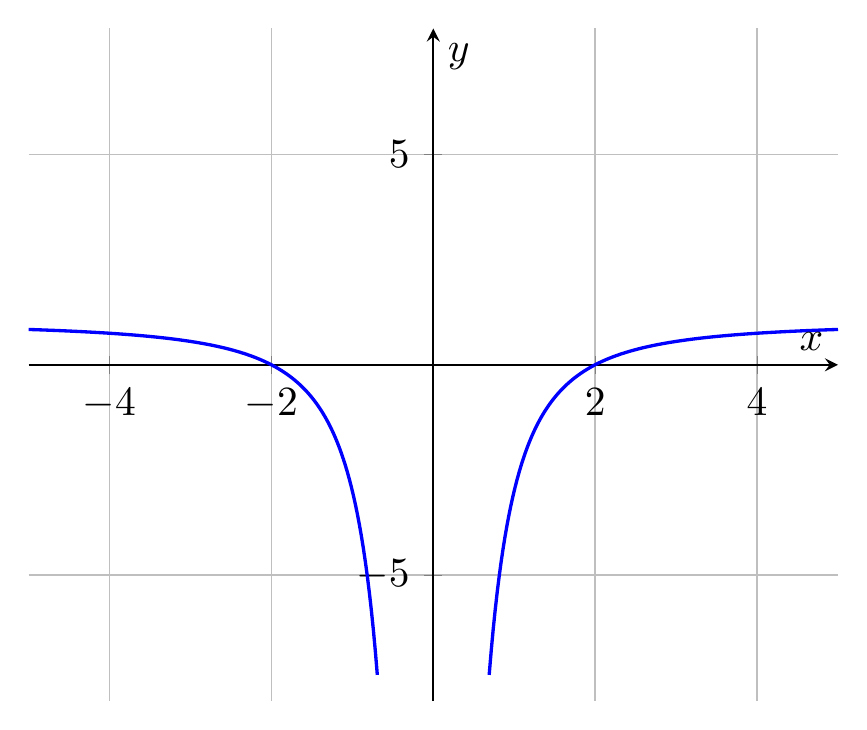
\begin{tikzpicture}[scale=1.5]
            \begin{axis}[
                axis lines=middle,
                grid=major,
                xmin=-5, xmax=5,
                ymin=-8, ymax=8,
                xlabel=$x$,
                ylabel=$y$,
                samples=200,
                restrict y to domain=-8:8,
                %discontinuities={-0.01, 0.01}
            ]
                \addplot[blue, thick, domain=-5:-0.1]{(x^2-4)/x^2};
                \addplot[blue, thick, domain=0.1:5]{(x^2-4)/x^2};
                
                % Vertical asymptote at x=0
                %\addplot[dashed, gray]{x/x * NaN};
                %\draw[dashed, gray] (0,-8) -- (0,8);
                
                % Horizontal asymptote at y=1
                %\draw[dashed, gray] (-5,1) -- (5,1);
            \end{axis}
        \end{tikzpicture}
    \end{image}
\end{exercise}

\begin{exercise}
    Sketch the graph of a function $g(x)$ that satisfies all of the following conditions: \\
    \begin{tabular}{c|c|c|c}
       Interval  & $g$ & $g'$ & $g''$  \\ \hline
        $(-\infty, -1)$ &  & $g'(x)>0$ & $g''(x)>0$\\
        x=-1 & 0 & DNE & DNE \\
        $(-1, 3)$ & & $g'(x)<0$ & $g''(x)>0$\\
        x=3 & -3 & 0 & $g''(x)>0$\\
        $(3,5)$ & & $g'(x)>0$ & $g''(x)>0$\\
        x=5 & 4 & $g'(x)>0 $& 0\\
        $(5,\infty)$ & & $g'(x)>0$ & $g''(x)<0$
    \end{tabular}
\end{exercise}

\begin{exercise}
    Find all intervals where the functions are increasing, decreasing, concave up, concave down.  Identify the location ($x$-value) for all local minima, maxima and inflection points (if any).   Sketch a graph using this information with one anchoring point.\\
\begin{enumerate}
    \item $f(x)=x^3-2x^2+x$
    \item $f(x)=x^2-8x^{\frac{1}{2}},\,\,\,\,\,\,\, (x\geq 0)$
    %\item $f(x)=x+\sin(x),\,\,\,\,\,\,\, x\in [0,2\pi]$
    \item $f(x)=(x^2-3)e^{-x}$ 
    \item $f(x)=\dfrac{x^3}{x+1}$
    
\end{enumerate}
\end{exercise}





\end{document}
